\documentclass[border=10pt]{standalone}

\usepackage{tikz}
\usepackage{tikzsymbols}
\usetikzlibrary{calc,patterns,shapes.geometric}

\def\centerarc[#1](#2)(#3:#4:#5){\draw[#1] ($(#2)+({#5*cos(#3)},{#5*sin(#3)})$) arc (#3:#4:#5);}

\begin{document}
	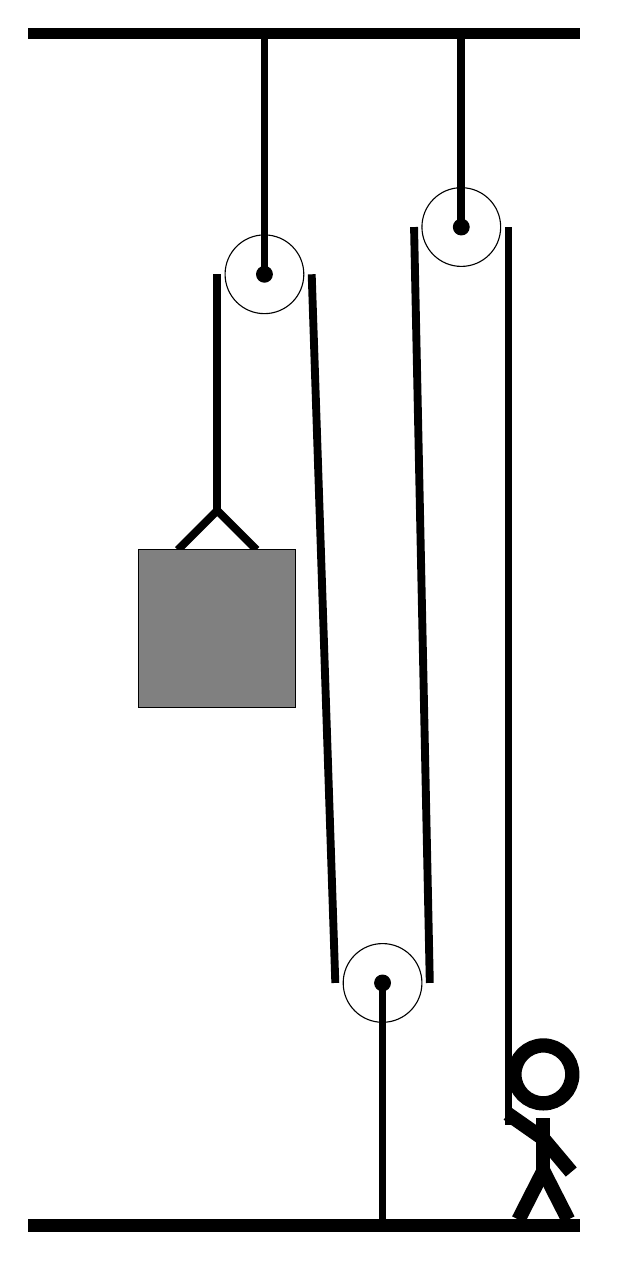
\begin{tikzpicture}
		%%%%% START %%%%%
		\draw[fill=black] (-2, 12) rectangle (5, 12.125);
		
		\draw (1, 9) circle (0.5);
		\draw[fill=black] (1, 9) circle (0.1);
		\draw[line width=1mm]  (1, 12) -- (1, 9);
		
		\draw[fill=white](2.5, 0) circle (0.5);
		\draw[fill=black] (2.5, 0) circle (0.1);
		\draw[line width=1mm]  (2.5, -3) -- (2.5, 0);
		
		\draw[fill=white](3.5, 9.6) circle (0.5);
		\draw[fill=black] (3.5, 9.6) circle (0.1);
		\draw[line width=1mm] (3.5, 12) -- (3.5, 9.6);
		
		\draw[line width=1mm] (-0.1, 5.5) -- (0.4, 6.0) -- (0.9, 5.5);
		\draw[fill=black!50] (-0.6, 5.5) rectangle (1.4, 3.5);
		
		\draw[line width=1mm] (0.4, 9) -- (0.4, 6.0);
		\centerarc[line width=1mm](1, 9)(0:180:0.6);
		\draw[line width=1mm](1.6, 9) -- (1.9, 0);
		\centerarc[line width=1mm](2.5, 0)(180:360:0.6);
		\draw[line width=1mm](3.1, 0) -- (2.9, 9.6);
		\centerarc[line width=1mm](3.5, 9.6)(0:180:0.6);
		\draw[line width=1mm](4.1, 9.6) -- (4.1, -1.8);
		
		\node at (4.5, -1.9) {\Strichmaxerl[10][-35][-50]};
		
		\draw[fill=black] (-2, -3) rectangle (5, -3.15);
		%%%%% END %%%%%
	\end{tikzpicture}
\end{document}